\chapter{Movimiento de partículas en un fluido}
\noindent
Fijado un espacio $\Omega\subseteq \mathbb{R}^3$, supondremos siempre que será abierto\footnote{Queremos estudiar movimientos de partículas en un fluido y pasan cosas no deseadas en la frontera.} y conexo\footnote{Por comodidad.}.

\begin{notacion}
    A cada punto de $\Omega$ lo notaremos normalmente por $p\in \Omega$, que tendrá coordenadas:
    \begin{equation*}
        p = (x,y,z)
    \end{equation*}
\end{notacion}

\noindent
El fluido suele llevar en cada punto una dirección y una velocidad, por lo que en cada punto $p\in \Omega$ tendremos un vector $v$ que determina la velocidad del fluido, la cual supondremos conocida siempre. Este vector no tiene por qué ser constante sino que puede depender del tiempo, por lo que generalmente $v$ será una función $v = v(t,p)$, es decir, $v:\mathbb{R}\times \Omega\to \mathbb{R}^3$ es una aplicación que a cada momento $t$ y posición $p$ le asigna un vector $v(t,p)$.\\

\noindent
Si tenemos una partícula en el fluido que se mueve esta determinará una trayectoria, que podemos modelar como una curva parametrizada $p(t)$.\\

\noindent
Podremos medir la velocidad de la partícula de dos formas: observando la velocidad de la partícula de forma interna (como el cuentakilómetros de un coche) o suponiendo que es una partícula que se deja llevar por la corriente y que su velocidad es la del fluido. La velocidad es la derivada de $p$.\\

\noindent
En el segundo caso:
\begin{equation*}
    \dot{p}(t) = V(t,p(t))
\end{equation*}
Estamos ante una ecuación diferencial. Observemos que es un sistema de primer orden en forma normal, puesto que las coordenadas de $p$ son funciones del tiempo. Si escribimos $V = (u,v,w)$ tenemos:
\begin{equation*}
    \left\{\begin{array}{l}
            \dot{x} = u(t,x,y,z) \\
            \dot{y} = v(t,x,y,z) \\
            \dot{z} = w(t,x,y,z)
    \end{array}\right.
\end{equation*}
Un sistema de 3 ecuaciones y 3 incógnitas, que conocidas las velocidades del fluido determina la trayectoria de la partícula. 

\begin{observacion}
    Observemos que en la notación primera hemos escrito explícitamente que $\dot{p}$ está en función de $t$. En la segunda notación estamos usando la notación habitual en las ecuaciones diferenciales, omitiendo la dependencia de $t$ y pensándola de forma implícita. Podemos así reescribir la primera ecuación como:
    \begin{equation*}
        \dot{p} = V(t,p)
    \end{equation*}
    Una vez denotamos $\dot{p}(t)$ estamos diciendo que es una solución concreta, por lo que será una variable dependiente de $t$. Sin embargo, cuando hablamos de $V(t,p)$ vemos $p$ como una variable independiente.
\end{observacion}

\noindent
Aparecerán sistemas autónomos, que representan fluidos estacionarios, donde la velocidad $V(t,p)$ no depende del tiempo.\\

\begin{ejemplo} % // TODO: Ver folio 1
    Comenzamos primero con dos ejemplos de fluidos estacionarios (el vector en cada posición no depende del tiempo):
    \begin{itemize}
        \item Consideramos $\Omega = \mathbb{R}^3$ y tomamos:
            \begin{equation*}
                V(t,x,y,z) = (0,1,0)
            \end{equation*}
            Observamos que es un sistema autónomo (no depende del tiempo) y en el que la velocidad tampoco depende de la posición:
            \begin{equation*}
                \left\{\begin{array}{l}
                        \dot{x} = 0 \\
                        \dot{y} = 1 \\
                        \dot{z} = 0 
                \end{array}\right.
            \end{equation*}
            Con lo que las soluciones son de la forma:
            \begin{align*}
                &x(t) = c_1 \\
                &y(t) = t + c_2 \\
                &z(t) = c_3
            \end{align*}
            Es una familia que depende de 3 parámetros.
        \item Tomamos la ecuación de un vórtice lineal, $\Omega = \mathbb{R}^3$ y:
            \begin{equation*}
                V(t,x,y,z) = (y, -x, 0)
            \end{equation*}
            Tenemos el sistema:
            \begin{equation*}
                \left\{\begin{array}{l}
                        \dot{x} = y \\
                        \dot{y} = -x \\
                        \dot{z} = 0
                \end{array}\right.
            \end{equation*}
            Es un sistema lineal homogéneo, que nos da las soluciones:
            \begin{align*}
                z(t) = c_3
            \end{align*}
            Reducimos a una ecuación de segundo orden, derivando en la primera:
            \begin{equation*}
                \ddot{x} + \dot{x} = 0
            \end{equation*}
            Por lo que:
            \begin{equation*}
                x(t) = c_1\cos(t) + c_2\sen(t)
            \end{equation*}
            Y también tendremos:
            \begin{equation*}
                y(t) = -c_1\sen(t) + c_2\cos(t)
            \end{equation*}
            Para ciertas condiciones iniciales $c_1,c_2,c_3\in \mathbb{R}$.
            % // TODO: Pensar por qué esto describe circunferencias
    \end{itemize}
\end{ejemplo}~\\

\noindent
Nuestro objetivo ahora es tratar de probar que el sistema:
\begin{equation*}
    \dot{p} = V(t,p)
\end{equation*}
con la condición inicial $p(t_0) = p_0$ tiene una solución. Luego trataremos de ver que en cada condición inicial tenemos una única solución. Demostraremos el Teorema de existencia y unicidad en cualquier número de dimensiones.

\begin{notacion}
    Notaremos a los puntos por $x=(x_1,\ldots,x_d)\in \mathbb{R}^d$ y al campo que define la ecuación diferencial por $X$, que será función de $t$ y de $x$, que estará definido en un conjunto $D\subseteq \mathbb{R}\times \mathbb{R}^d$ y exigiremos que sea abierto y conexo. Así, tendremos
    \Func{X}{D}{\bb{R}^d}{(t,x)}{X(t,x)}
    donde el campo $X$ tiene $d$ coordenadas:
    \begin{equation*}
        X = (X_1, \ldots, X_d)
    \end{equation*}
    donde tratamos de resolver la ecuación $\dot{x} = X(t,x)$, que en realidad es un sistema de ecuaciones:
    \begin{equation*}
        \left\{\begin{array}{l}
                \dot{x_1} = X_1(t,x_1,\ldots,x_d) \\
                \vdots \\
                \dot{x_d} = X_d(t,x_1,\ldots,x_d) 
        \end{array}\right.
    \end{equation*}
    Supondremos siempre que $X$ es una función continua.\\

    \noindent
    Tomaremos $(t_0,x_0) \in D$ y queremos resolver el problema de condiciones iniciales
    \begin{equation*}
        \dot{x} = X(t,x), \qquad x(t_0) = x_0
    \end{equation*}
    que consiste en resolver la ecuación diferencial superior mediante una solución que cumpla la condición enunciada.
\end{notacion}~\\

\section{Problema a resolver}
\noindent
Así, queremos resolver el problema:
\begin{equation}\label{eq:problema}
    \dot{x} = X(t,x)
\end{equation}
con $X:D\to \mathbb{R}^d$ continuo, donde $D\subset \mathbb{R}\times\mathbb{R}^d$ es un subconjunto abierto y conexo. La condición de que $X$ sea continuo es equivalente a que cada una de sus coordenadas
\begin{equation*}
    X = (X_1,\ldots,X_d)
\end{equation*}
sea una aplicación continua.

\begin{definicion}
    Una \textbf{solución} del problema~\eqref{eq:problema} es una aplicación $x:I\to \mathbb{R}^d$ donde  $I\subset \mathbb{R}$ es un intervalo\footnote{No necesariamente abierto.} de forma que $x(t)\subset D$:
    \begin{enumerate}
        \item[$i)$] $x(t)$ es derivable.
        \item[$ii)$] $(t,x(t))\in D\qquad \forall t\in I$.
        \item[$iii)$] $\dot{x}(t) = X(t,x(t)) \qquad \forall t\in I$.
    \end{enumerate}
\end{definicion}

\begin{observacion}
    Observemos que la definición de solución del problema planteado anteriormente es equivalente si sustituimos la condición de que $x$ sea derivable por la condición de que $x$ sea de clase 1, puesto que la condición $iii)$ nos da automáticamente la continuidad de la derivada de $x$. 

    \noindent
    Así, la condición $i)$ se puede sustituir por la condición $i')~x\in C^1(I,\mathbb{R}^d)$.
\end{observacion}

\begin{ejemplo}
    Veamos un par de ejemplos para fijar las ideas:
    \begin{enumerate}
        \item Consideramos $\dot{x} = x^2$ y la aplicación $x(t) = \dfrac{1}{1-t}$. Vamos a analizar el marco del problema.

            Tenemos en este caso $d=1$ y $D=\mathbb{R}^2$, puesto que tenemos el campo vectorial $X(t,x) = x^2$, que es continuo en todo $D=\mathbb{R}\times \mathbb{R}$. 

            Tenemos una primera solución en $I_1 = \left]-\infty,1\right[$, $x_1(t) = \frac{1}{1-t}$.

            Y otra solución en $I_2 = \left]1,+\infty\right[$, $x_2(t) = \frac{1}{1-t}$.

            Son \underline{dos soluciones distintas}, con la misma fórmula.
        \item Consideramos ahora $\dot{x} = \frac{x}{t}$ y la aplicación $x(t) = -7t$.

            Tenemos $d=1$ y el campo es $X(t,x) = \frac{x}{t}$, que tiene dos posibles dominios de definición:
            \begin{equation*}
                D_1 = \mathbb{R}^-\times \mathbb{R}, \qquad D_2 = \mathbb{R}^+\times \mathbb{R}
            \end{equation*}
            Tenemos en realidad dos ecuaciones diferenciales.

            Para discutir una de sus soluciones, si consideramos:
            \begin{equation*}
                I_1 = \mathbb{R}^-, \qquad I_2 = \mathbb{R}^+
            \end{equation*}
            tenemos que $x\big|_{I_1}$ es solución de la ecuación diferencial considerando el dominio $D_1$ y análogamente para $x\big|_{I_2}$ con el dominio $D_2$.
    \end{enumerate}
\end{ejemplo}

\noindent
Para una ecuación $\dot{x} = X(t,x)$ definida en un dominio $D\subset\mathbb{R}\times \mathbb{R}^d$ abierto y conexo, acompañaremos usualmente la ecuación de una \textbf{condición inicial}, que es fijar un punto $(t_0,x_0)\in D$ y obligaremos a la solución $x(t)$ de la ecuación que verifique la condición:
\begin{equation}\label{eq:condicion_inicial}
    x(t_0) = x_0
\end{equation}
Cuando nos refiramos próximamente al problema~\eqref{eq:problema} nos estaremos refiriendo usualmente a un problema de valores iniciales dado por la fórmula destacada y por la condición~\eqref{eq:condicion_inicial}.

\begin{ejemplo}
    En el primer ejemplo anterior tenemos para la condición inicial $x(0) = 1$ que la solución de $\dot{x} = x^2$ es $x:\left]-\infty,1\right[\to \mathbb{R}$ dada por:
    \begin{equation*}
        x(t) = \frac{1}{1-t}
    \end{equation*}
\end{ejemplo}

\begin{teo}[Cauchy-Peano, Existencia de soluciones de ecuaciones diferenciales.]\label{teo:existencia}
    Todo problema de valores iniciales admite una solución definida en algún intervalo\footnote{Por tanto, el Teorema nos da una solución local.} $I$ con $t_0\in \mathring{I}$.
\end{teo}

\begin{observacion}
    El ejepmlo anterior nos demuestra que el Teorema de Cauchy-Peano no puede generalizarse a otro que resuelva el problema de forma global, puesto que tenemos una solución para la ecuación que no puede extenderse a todo $\mathbb{R}$; a pesar de ser el dominio de la ecuación todo $\mathbb{R}^2$.
\end{observacion}

\noindent
Lo que venga a continuación estará destinado a probar el Teorema anterior.\\

\noindent
El primer paso será pasar el problema de valores iniciales a una ecuación integral, puesto que la ecuación diferencial y el problema de condiciones iniciales son muy intuitivos pero difíciles de manipular desde el punto de vista de las demostraciones.

\section{Ecuación integral de Volterra}
La ecuación integral de Volterra es:
\begin{equation}\label{eq:Volterra}
    x(t) = x_0 + \int_{t_0}^{t} X(s,x(s))~ds 
\end{equation}
Es la ecuación que obtenemos al integrar $\dot{x} = X(t,x)$. Así, a cada ecuación diferencial podemos asociarle una ecuación de Volterra y a cada ecuación de Volterra podemos asociarle una ecuación diferencial.

\begin{ejemplo}
    El problema de valores iniciales $\dot{x} = 3x$ con la condición inicial $x(2) = -5$ tiene ecuación integral de Volterra:
    \begin{equation}\label{eq:ejmVolterra}
        x(t) = -5 + \int_{2}^{t} 3x(s)~ds 
    \end{equation}
\end{ejemplo}

\begin{definicion}
    Una solución de~\eqref{eq:Volterra} es una función $x:I\to \mathbb{R}^d$ con $I$ un intervalo que contiene a $t_0$ en su interior y:
    \begin{enumerate}
        \item[$i)$] $x$ es continua.
        \item[$ii)$] $(t,x(t)) \in D\qquad \forall t\in I$.
        \item[$iii)$] Se cumple la condición~\eqref{eq:Volterra} para todo $t\in I$.
    \end{enumerate}
\end{definicion}

\begin{ejemplo}
    Una solución de la ecuación integral de Volterra~\eqref{eq:ejmVolterra} es:
    \begin{equation*}
        x(t) = -5e^{3(t-2)} \qquad \forall t\in \mathbb{R}
    \end{equation*}
\end{ejemplo}

\noindent
La estrategia será enunciar los Teoremas como ecuaciones diferenciales y realizar sus demostraciones con ecuaciones integrales.

\begin{prop}
    Los problemas~\eqref{eq:problema} y~\eqref{eq:Volterra} son equivalentes\footnote{Es decir, tienen las mismas soluciones.}.
    \begin{proof}
        Supondremos que tenemos una solución de una ecuación y tendremos que probar entonces que tenemos una solución de la otra ecuación. Basta aplicar el Teorema Fundamental del Cálculo en un caso y la Regla de Barrow en el otro.
        \begin{itemize}
            \item Supuesto que $x:I\to \mathbb{R}^d$ es solución de la ecuación~\eqref{eq:problema}, tenemos entonces que $x$ es una aplicación derivable que verifica\footnote{Observemos que la condición $ii)$ en el primer caso es equivalente a la condición $ii)$ del segundo caso.}:
                \begin{equation*}
                    \dot{x}(t) = X(t,x(t)) \qquad \forall t\in I
                \end{equation*}
                Por lo que $\dot{x}$ es una primitiva de la aplicación $t\mapsto X(t,x(t))$ definida en $I$, que sabemos que es continua. La Regla de Barrow nos dice entonces que fijado $t_0\in I$ se tiene:
                \begin{equation*}
                    \int_{t_0}^{t} X(s,x(s))~ds = x(t) - x(t_0) = x(t) - x_0 \qquad \forall t\in I
                \end{equation*}
                Y despejando obtenemos~\eqref{eq:Volterra}.
            \item Supuesto que $x:I\to \mathbb{R}^d$ es solución de la ecuación~\eqref{eq:Volterra}, tenemos en este caso que $x$ es una aplicación continua que verifica:
                \begin{equation*}
                    x(t) = x_0 + \int_{t_0}^{t} X(s,x(s))~ds  \qquad \forall t\in I
                \end{equation*}
                Como $x$ es continua, la aplicación $s\mapsto X(s,x(s))$ y de dominio $I$ será también continua. Bajo estas hipótesis, el Teorema Fundamental del Cálculo nos dice que la aplicación
                \begin{equation*}
                    t\longmapsto \int_{t_0}^{t} X(s,x(s))~ds 
                \end{equation*}
                de dominio $I$ es derivable, por lo que también lo será la aplicación $x$, y su derivada es:
                \begin{equation*}
                    \dot{x}(t) = X(t,x(t)) \qquad \forall t\in I
                \end{equation*}
                Hemos obtenido que $x$ es solución de~\eqref{eq:problema}, y es claro que $x(t_0) = x_0$.
        \end{itemize}
    \end{proof}
\end{prop}

\subsection{El Teorema global}
\noindent
La estrategia a seguir será probar un Teorema global con hipótesis extra para luego retringir el problema y obtener la demostración del Teorema local.

\begin{teo}[global de existencia]\label{teo:global_existencia}
    Sea $D=\left]a,b\right[\times \mathbb{R}^d$ para ciertos $a,b\in \mathbb{R}$ y $X:\left]a,b\right[\times \mathbb{R}^d\to \mathbb{R}^d$ continuo de forma que
    \begin{equation*}
        \exists M>0 : \|X(t,x)\|\leq M \qquad \forall (t,x)\in D
    \end{equation*}
    Entonces~\eqref{eq:problema} tiene una solución definida en todo el intervalo $\left]a,b\right[$.
\end{teo}

\begin{ejemplo}
    Familiaricémonos con este problema.
    \begin{enumerate}
        \item Consideramos el sistema
            \begin{equation*}
                \left\{\begin{array}{ll}
                     \dot{x}_1 = \dfrac{x_2}{1+x_2^2 + x_1^2} + t\sen(x_1),& \qquad x_1(0) = 3 \\
                                                                           &\\
                     \dot{x}_2 = e^{-x_1^2} + \sqrt{1-t^2},& \qquad x_2(0) = 7 \\
                \end{array}\right. 
            \end{equation*}
            Aquí tenemos $d=2$, $\left]a,b\right[ = \left]-1,1\right[$, con $X:\left]-1,1\right[\times \mathbb{R}^2\to \mathbb{R}^2$ continuo.

            Veamos que $X$ está acotado, como todas las normas son equivalentes, tomaremos la norma del máximo: $\|(x_1,x_2)\| = \max\{|x_1|,|x_2|\}$:
            \begin{align*}
                \|X(t,x)\| &\leq\max\left\{2,2\right\} = 2 \qquad \forall (t,x)\in \left]-1,1\right[\times \mathbb{R}^2
            \end{align*}
            Tenemos además que $t_0 = 0\in \left]a,b\right[$ así como que $x_0 = (3,7) \in \mathbb{R}^2$.
        \item Veamos ahora que la hipótesis de que $X$ es acotado es esencial, puesto que el problema de valores iniciales $\dot{x} = x^2$, $x(0) = 1$ con solución
            \begin{equation*}
                x(t) = \frac{1}{1-t}, \qquad t\in \left]-3,1\right[
            \end{equation*}
            donde tenemos\footnote{Podríamos haber tomado $D=\mathbb{R}\times \mathbb{R}$, pero queremos verificar las hipótesis del Teorema.} $D=\left]-3,3\right[\times \mathbb{R}$. Próximamente veremos que esta solución es la única para la condición inicial enunciada, lo que nos garantizará que esta solución no puede extenderse a otra que esté definida en $\left]-3,3\right[$.
    \end{enumerate}
\end{ejemplo}

\noindent
Vamos a ver a continuación que el Teorema~\ref{teo:existencia} puede deducirse a partir del Teorema~\ref{teo:global_existencia}, por lo que nuestro futuro trabajo será probar este segundo. Para probar esta relación usaremos el Lema del Pegado, que ya conocíamos de Topología I.

\begin{lema}\label{lema:del_pegado}
    Sean $X,Y$ espacios métricos y $F_1,F_2\subset X$ dos cerrados de forma que $F_1\cup F_2 = X$. Sean $f_i:F_i\to Y$ continuas para $i \in \{1,2\}$ verificando que $f_1 = f_2$ en $F_1\cap F_2$. Entonces la función $f:X\to Y$ dada por:
    \begin{equation*}
        f(x) = \left\{\begin{array}{ll}
            f_1(x) & \text{si\ } x\in F_1 \\
            f_2(x) & \text{si\ } x\in F_2
        \end{array}\right. 
    \end{equation*}
    está bien definida y es continua.
\end{lema}

\begin{prop}
    Del Teorema~\ref{teo:global_existencia} puede deducirse el Teorema~\ref{teo:existencia}.
    \begin{proof} 
        Como $D$ es abierto y $(t_0,x_0)\in D$, podemos tomar $a,b>0$ de forma que:
        \begin{equation*}
            R = \{(t,x)\in \mathbb{R}\times\mathbb{R}^d : |t-t_0|\leq a, \|x-x_0\|\leq b\} \subset D
        \end{equation*} 
        \begin{figure}[H]
            \centering
            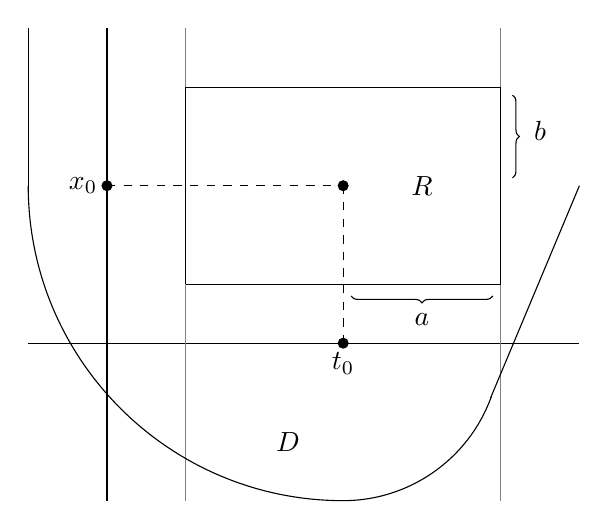
\begin{tikzpicture}
            \draw (-1,0) -- (6,0);
            \draw (0,-2) -- (0,4);
            \fill (0,2) circle(2pt) node[left] {$x_0$};
            \fill (3,0) circle(2pt) node[below] {$t_0$};
            \fill (3,2) circle(2pt) node[] {};
            \fill (4,2) node[] {$R$};
            \draw[dashed] (0,2) -- (3,2);
            \draw[dashed] (3,0) -- (3,2);
            \draw[gray] (1,-2) -- (1,4);
            \draw[gray] (5,-2) -- (5,4);
            \draw (1,0.75) -- (1,3.25);
            \draw (5,0.75) -- (5,3.25);
            \draw (1,0.75) -- (5,0.75);
            \draw (1,3.25) -- (5,3.25);

            \draw (3,2) ++(180:4) arc (180:270:4);
            \draw (-1,2) -- (-1,4);
            \draw (3,0) ++(270:2) arc (270:340:2);
            \draw (4.87,-0.7) -- (6,2);
            \fill (2.3,-1.5) node[above] {$D$};

            \draw[decorate, decoration={brace, mirror}] (3.1,0.6) -- (4.9,0.6);
            \fill (4,0.30) node[] {$a$};
            \draw[decorate, decoration={brace}] (5.15,3.15) -- (5.15, 2.1);
            \fill (5.5, 2.7) node[] {$b$};
            \end{tikzpicture}
        \end{figure}
        \noindent
        Nuestro objetivo es tratar de extender el campo $X$ definido en el conjunto $D$ a toda la banda $\left]t_0-a,t_0+a\right[\times \mathbb{R}^d$. Inicialmente podríamos pensar en asignarle el valor $0$ fuera de la región $R$, pero entonces podríamos perder la continuidad del campo $X$. Este problema tiene fácil arreglo, pues basta reservar una zona en la que ``unir'' el campo $X$ con la función constantemente igual a cero de forma continua. Para ello, tomaremos $0<b^\ast<b$ y consideraremos:
        \begin{equation*}
            R^\ast = \{(t,x)\in \mathbb{R}\times\mathbb{R}^d : |t-t_0|\leq a, \|x-x_0\|\leq b^\ast\} \subset D
        \end{equation*} 
        \begin{figure}[H]
            \centering
            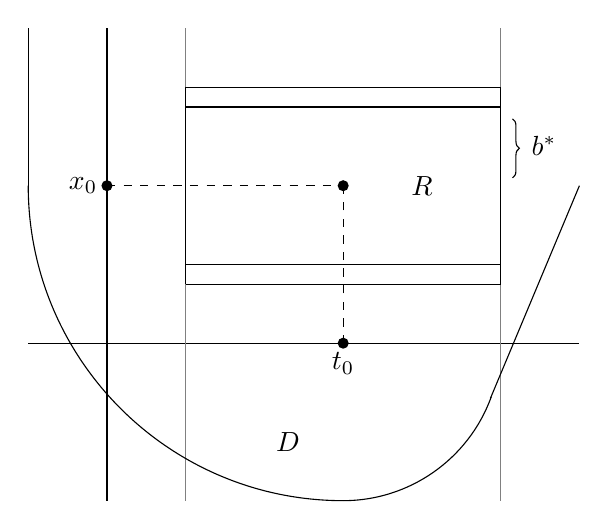
\begin{tikzpicture}
            \draw (-1,0) -- (6,0);
            \draw (0,-2) -- (0,4);
            \fill (0,2) circle(2pt) node[left] {$x_0$};
            \fill (3,0) circle(2pt) node[below] {$t_0$};
            \fill (3,2) circle(2pt) node[] {};
            \fill (4,2) node[] {$R$};
            \draw[dashed] (0,2) -- (3,2);
            \draw[dashed] (3,0) -- (3,2);
            \draw[gray] (1,-2) -- (1,4);
            \draw[gray] (5,-2) -- (5,4);
            \draw (1,0.75) -- (1,3.25);
            \draw (5,0.75) -- (5,3.25);
            \draw (1,0.75) -- (5,0.75);
            \draw (1,3.25) -- (5,3.25);

            \draw (3,2) ++(180:4) arc (180:270:4);
            \draw (-1,2) -- (-1,4);
            \draw (3,0) ++(270:2) arc (270:340:2);
            \draw (4.87,-0.7) -- (6,2);
            \fill (2.3,-1.5) node[above] {$D$};

            \draw (1,1) -- (5,1);
            \draw (1,3) -- (5,3);
            \draw[decorate, decoration={brace}] (5.15,2.85) -- (5.15, 2.1);
            \fill (5.55, 2.5) node[] {$b^\ast$};
            \end{tikzpicture}
        \end{figure}
        \noindent
        Definimos $\psi:\left]t_0-a,t_0+a\right[\times \mathbb{R}^d\to \mathbb{R}$ continua de forma que:
        \begin{gather*}
            \psi = 1 \quad \text{en}\quad \|x-x_0\| < b^\ast \\
            \psi = 0 \quad \text{en}\quad \|x-x_0\| > b \\
            0\leq \psi \leq 1 \quad \text{siempre}
        \end{gather*}
        Y definimos el campo modificado $X^\ast:\left]t_0-a,t_0+a\right[\times \mathbb{R}^d\to \mathbb{R}^d$ dado por:
        \begin{equation*}
            X^\ast(t,x) = \left\{\begin{array}{ll}
                \psi(t,x)\cdot X(t,x) & \text{si\ }\|x-x_0\|\leq b  \\
                 0 & \text{si\ } \|x-x_0\| > b
            \end{array}\right. 
        \end{equation*}
        Vemos que $X(t,x) = X^\ast(t,x)$ para todo $(t,x)\in R^\ast$.\\

        \noindent
        Buscamos aplicar ahora el Teorema~\ref{teo:global_existencia} a $\dot{x} = X^\ast(t,x)$, $x(t_0) = x_0$. Falta comprobar la contiuidad de $X^\ast$ y su acotación.

        \begin{itemize}
            \item Para la contuidad de $X^\ast$, si consideramos en el espacio $\left]t_0-a,t_0+a\right[\times \mathbb{R}^d$:
                \begin{align*}
                    F_1 &= \{(t,x)\in \mathbb{R}\times \mathbb{R}^d : |t-t_0|<a, \|x-x_0\| \leq b\} \\
                    F_2 &= \{(t,x)\in \mathbb{R}\times \mathbb{R}^d : |t-t_0|<a, \|x-x_0\| \geq b\} 
                \end{align*}
                Vemos que definiendo $f_1 = \psi \cdot X$, $f_2 = 0$ se tiene que\footnote{Por la contiuidad de $\psi$ tenemos que $\psi(x) = 0$ cuando $\|x-x_0\| = b$.} $f_1 = f_2$ en $F_1\cap F_2$. Aplicando el Lema~\ref{lema:del_pegado} obtenemos que la función $X^\ast$ es continua.
            \item $X$ es continuo y $R\subset D$ es compacto, por lo que:
                \begin{equation*}
                    \exists M>0 : \|X(t,x)\|\leq M \qquad \forall (t,x)\in R
                \end{equation*}
                Como $\psi \leq 1$ obtenemos que $X^\ast$ es también acotada a partir de su definición.
        \end{itemize}
        Aplicando ahora el Teorema~\ref{teo:global_existencia} obtenemos que existe $x:\left]t_0-a,t_0+a\right[\to \mathbb{R}^d$ que es solución del problema:
        \begin{equation*}
            \dot{x}(t) = X^\ast(t,x(t)), \qquad x(t_0) = x_0
        \end{equation*} 
        Vemos que $x(t)$ no puede (quizás) ser solución del problema planteado con el campo $X$ en el dominio $D$. 
        \begin{figure}[H]
            \centering
            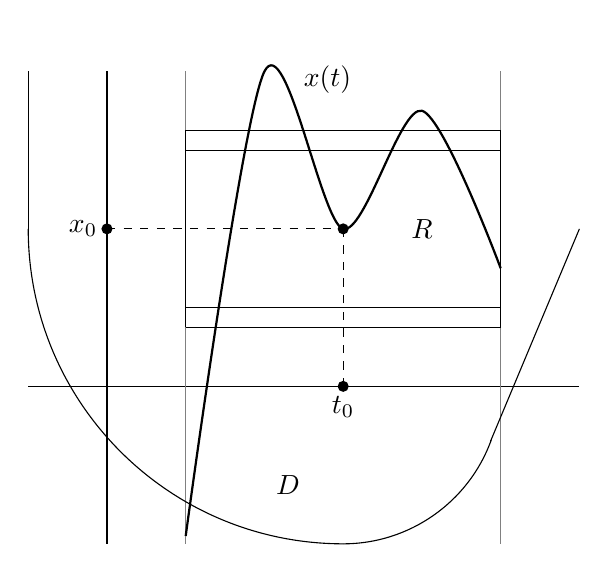
\begin{tikzpicture}
            \draw (-1,0) -- (6,0);
            \draw (0,-2) -- (0,4);
            \fill (0,2) circle(2pt) node[left] {$x_0$};
            \fill (3,0) circle(2pt) node[below] {$t_0$};
            \fill (3,2) circle(2pt) node[] {};
            \fill (4,2) node[] {$R$};
            \draw[dashed] (0,2) -- (3,2);
            \draw[dashed] (3,0) -- (3,2);
            \draw[gray] (1,-2) -- (1,4);
            \draw[gray] (5,-2) -- (5,4);
            \draw (1,0.75) -- (1,3.25);
            \draw (5,0.75) -- (5,3.25);
            \draw (1,0.75) -- (5,0.75);
            \draw (1,3.25) -- (5,3.25);

            \draw (3,2) ++(180:4) arc (180:270:4);
            \draw (-1,2) -- (-1,4);
            \draw (3,0) ++(270:2) arc (270:340:2);
            \draw (4.87,-0.7) -- (6,2);
            \fill (2.3,-1.5) node[above] {$D$};

            \draw (1,1) -- (5,1);
            \draw (1,3) -- (5,3);

            \fill (2.8,3.9) node[] {$x(t)$};
            % Spline que pasa por ciertos puntos
            \draw[thick] plot[smooth] coordinates {
                    (1,-1.9)
                    (2,4)
                    (3,2)
                    (4,3.5)
                    (5,1.5)
            };
            \end{tikzpicture}
        \end{figure}


        \noindent
        Sin embargo, sí que nos podemos restringir a un entorno en el que sea solución. Tenemos que:
        \begin{gather*}
            \dot{x}(t) = X(t,x) = X^\ast(t,x) \quad \text{si}\quad \|x-x_0\| < b^\ast \\
            x(t_0) = x_0, \quad \qquad x(t)\quad \text{continua}
        \end{gather*}
        Y además:
        \begin{equation*}
            \exists \delta>0 : \|x(t)-x_0\| < b^\ast \qquad \forall t\in [t_0-\delta,t_0+\delta]
        \end{equation*}
        Con lo que $x\big|_{[t_0-\delta,t_0+\delta]}$ sí que es solución de $\dot{x} = X(t,x)$, $x(t_0) = x_0$.
    \end{proof}
\end{prop}

\subsection{Demostración del Teorema global}
\noindent
Nuestro interés será ahora probar el Teorema~\ref{teo:global_existencia}. Recordando las hipótesis, tenemos una función $X:\left]a,b\right[\times \mathbb{R}^d\to \mathbb{R}^d$ continuo y acotado:
\begin{equation*}
    \exists M:\|X(t,x)\|\leq M \qquad \forall (t,x)\in \left]a,b\right[\times \mathbb{R}^d
\end{equation*}
Así como $t_0\in \left]a,b\right[$ y $x_0\in \mathbb{R}^d$. Queremos llegar a probar que existe una solución definida en $\left]a,b\right[$ de $\dot{x} = X(t,x)$, $x(t_0) = x_0$.\\

\noindent
La demostración se dividirá en 3 etapas:

\begin{description}
    \item [1 - Construcción de soluciones aproximadas.] Fijado $\varepsilon>0$, definiremos \newline $x_{\varepsilon}:\left]a,b\right[\to \mathbb{R}^d$ continua de forma que se verifica\footnote{La constante $M\varepsilon$ es por comodidad, se podría haber sustituido por $\varepsilon$.}:
        \begin{equation*}
            \left\|x_{\varepsilon} -x_0- \int_{t_0}^{t} X(s,x(s))~ds \right\| \leq M \varepsilon \qquad \forall t\in \left]a,b\right[
        \end{equation*}
        Estas funciones $x_{\varepsilon}$ serán soluciones aproximasdas a la ecuación de Volterra que estamos buscando, y seguiremos el método de Tonelli para construirlas.
    \item [2 - Argumento de compacidad (Ascoli-Arzelà).] En esta etapa queremos pasar al límite de una sucesión de aproximaciones $x_{\varepsilon_n}$, que queremos que tengan límite, para lo que nos serán de especial relevancia los conjuntos compactos en un espacio de funciones. La convergencia que nos interesará será la convergencia uniforme.
    \item [3 - Paso al límite.] Tendiendo $n$ a infinito obtendremos la solución como límite de la sucesión construida.
\end{description}

% // TODO: Meter idea de Tonelli

\begin{ejemplo}
    Consideramos $x'=\sen x$, $x(0) = \frac{\pi}{2}$, $[0,2]$ y $\varepsilon=1$. La solución aproximada sería:
    \begin{equation*}
        x_1(t) = \left\{\begin{array}{ll}
                \dfrac{\pi}{2} & \text{si\ } t\in [0,1] \\
                              & \\
                \displaystyle \frac{\pi}{2}+\int_{0}^{t-1} \sen x_1(s)~ds = \frac{\pi}{2}+\int_{0}^{t-1}ds = \frac{\pi}{2}+t-1 & \text{si\ } t\in [1,2]
        \end{array}\right. 
    \end{equation*}
\end{ejemplo}

\subsubsection{1 - Construcción de soluciones aproximadas}
\noindent
Sea $\varepsilon>0$ cumpliendo $\varepsilon<\min(t_0-a,b-t_0)$ (así $[t_0-\varepsilon,t_0+\varepsilon]\subset \left]a,b\right[$), definimos $x_{\varepsilon}:\left]a,b\right[\to \mathbb{R}^d$ dada por:
\begin{equation*}
    x_\varepsilon(t) = \left\{\begin{array}{ll}
            x_0 & \text{si\ } t\in [t_0-\varepsilon,t_0+\varepsilon] \\
            \displaystyle x_0 + \int_{t_0}^{t-\varepsilon} X(s,x_{\varepsilon}(s))~ds & \text{si\ } t\in \left]t_0+\varepsilon,b\right[ \\
                                                                                      & \\
            \displaystyle x_0 + \int_{t_0}^{t+\varepsilon} X(s,x_{\varepsilon}(s))~ds & \text{si\ } t\in \left]a,t_0-\varepsilon\right[
    \end{array}\right. 
\end{equation*}
Es fácil ver que $x_{\varepsilon}$ está bien definida y que es continua, pues la definición en cierto intervalo depende de la definición de la función en otro intervalo y el intervalo inicial a considerar es $[t_0-\varepsilon,t_0+\varepsilon]$, donde las soluciones aproximadas comienzan tomando un valor de $x_0$.
\begin{figure}[H]
    \centering
    \begin{tikzpicture}
    \draw (0,0) -- (10,0);
    \fill (0,0) circle(2pt) node[below] {$a$};
    \fill (10,0) circle(2pt) node[below] {$b$};
    \fill (4,0) circle(2pt) node[below] {$t_0$};
    \fill[blue] (3,0) circle(2pt) node[above] {$t_0-\varepsilon$};
    \fill[blue] (5,0) circle(2pt) node[above] {$t_0+\varepsilon$};
    \fill[blue] (2,0) circle(2pt) node[] {};
    \fill[blue] (6,0) circle(2pt) node[] {};
    \fill[blue] (1,0) circle(2pt) node[] {};
    \fill[blue] (7,0) circle(2pt) node[] {};
    \fill[blue] (8,0) circle(2pt) node[] {};
    \fill[blue] (9,0) circle(2pt) node[] {};

    \draw[decorate, decoration={brace, mirror}] (3,-0.75) -- (5, -0.75);
    \fill (4,-1.2) node[] {$x_{\varepsilon}(t) = x_0$};

    \fill[gray] (6.5,0) circle(1.5pt) node[] {};
    \fill[gray] (5.5,0) circle(1.5pt) node[] {};
    \fill[gray] (4.5,0) circle(1.5pt) node[] {};

    \draw[-Stealth, gray, bend left=60] (6.5,0) to (5.55,-0.1);
    \draw[-Stealth, gray, bend left=60] (5.5,0) to (4.55,-0.1);
    \end{tikzpicture}
\end{figure}

\noindent
Veamos ahora que son soluciones aproximadas, es decir, que:
\begin{equation*}
    \|E(t)\| = \left\|x_{\varepsilon} -x_0- \int_{t_0}^{t} X(s,x(s))~ds \right\| \leq M \varepsilon \qquad \forall t\in \left]a,b\right[
\end{equation*}

Para ello:
\begin{itemize}
    \item Si $t\in [t_0-\varepsilon,t_0+\varepsilon]$ tenemos que:
        \begin{equation*}
            \|E(t)\| = \left\|\int_{t_0}^{t} X(s,x_0)~d \right\| \leq \left|\int_{t_0}^{t} \|X(s,x_0)\|~ds \right| \leq M|t-t_0| \leq M\varepsilon
        \end{equation*}
    \item Si $t\in \left]t_0+\varepsilon,b\right[$:
        \begin{align*}
            \|E(t)\| &= \left\|x_{\varepsilon}(t)-x_0-\int_{t_0}^{t-\varepsilon}X(s,x_{\varepsilon}(s))~ds - \int_{t-\varepsilon}^{t} X(s,x_{\varepsilon}(s))~ds  \right\| \\ 
                     &= \left\|\int_{t-\varepsilon}^{t} X(s,x_{\varepsilon}(s))~ds \right\| \leq \int_{t-\varepsilon}^{t} \|X(s,x_{\varepsilon}(s))\|~ds  \leq M\varepsilon
        \end{align*}
\end{itemize}

\subsubsection{2 - Argumento de compacidad (Ascoli-Arzelà)}
\noindent
Abstrayendo el problema actual a un marco general, trabajaremos con un intervalo $I\subset \mathbb{R}$ y una sucesión de funciones $f_n:I\to \mathbb{R}^d$. Sea $f:I\to \mathbb{R}^d$, diremos que $f_n\to f$ \textbf{converge uniformemente} si:
\begin{equation*}
    \forall \varepsilon>0~\exists N\in \mathbb{N} : n>N \quad\Longrightarrow\quad \|f_n(t)-f(t)\| < \varepsilon \qquad \forall t\in I
\end{equation*}
La idea que hay detrás es que para cada error $\varepsilon$ existe un término suficientemente avanzado de forma que toda la sucesión se queda dentro de un ``tubo'' de radio $\varepsilon$ alrededor de la gráfica de la función $f$ que aproximamos:
\begin{figure}[H]
    \centering
    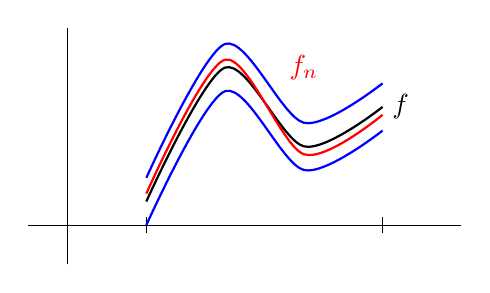
\begin{tikzpicture}
    \draw (0,-0.5) -- (0,2.5);
    \draw (-0.5,0) -- (5,0);
    \draw (1,-0.1) -- (1,0.1);
    \draw (4,-0.1) -- (4,0.1);

    % Spline que pasa por ciertos puntos
    \draw[thick] plot[smooth] coordinates {
            (1,0.3)
            (2,2)
            (3,1)
            (4,1.5)
    };
    \fill (4,1.5) node[right] {$f$};

    \draw[thick, red] plot[smooth] coordinates {
            (1,0.4)
            (2,2.1)
            (3,0.9)
            (4,1.4)
    };
    \fill[red] (3,2) node[] {$f_n$};

    \draw[thick, blue] plot[smooth] coordinates {
            (1,0.6)
            (2,2.3)
            (3,1.3)
            (4,1.8)
    };

    \draw[thick, blue] plot[smooth] coordinates {
            (1,0)
            (2,1.7)
            (3,0.7)
            (4,1.2)
    };
    \end{tikzpicture}
\end{figure}
\noindent
Por otra parte, decimos que $f_n\to f$ \textbf{converge puntualmente} si:
\begin{equation*}
    \forall \varepsilon>0~~\forall t\in I~~\exists N\in \mathbb{N}~~:~~n>N \quad\Longrightarrow\quad \|f_n(t)-f(t)\| < \varepsilon 
\end{equation*}
Con lo que la constante $N$ que encontramos cada vez depende ahora del punto $t\in I$ en el que nos encontramos.

\begin{ejemplo} 
    Sea $f_n:[0,1]\to \mathbb{R}$ cuya gráfica es para cada $n\in \mathbb{N}$ la de un triángulo de base $\nicefrac{1}{n}$, altura $1$ y que vale $0$ en el resto de su dominio:
    \begin{figure}[H]
        \centering
        \begin{tikzpicture}
        \draw (0,0) -- (0,3);
        \draw (0,0) -- (3.5,0);
        \draw[thick, blue] (0,0) -- (0.5,2.5);
        \draw[thick, blue] (0.5,2.5) -- (1, 0);
        \draw[thick, blue] (1,0) -- (2.5,0);

        \draw (-0.1, 2.5) -- (0.1, 2.5);
        \fill (-0.1, 2.5) node[left] {$1$};

        \draw (0.5, -0.1) -- (0.5, 0.1);
        \fill (0.5, -0.1) node[below] {$\frac{1}{2n}$};
        \draw[dashed] (0.5,2.5) -- (0.5,0);

        \draw (2.5, -0.1) -- (2.5, 0.1);
        \fill (2.5, -0.1) node[below] {$1$};
        \end{tikzpicture}
    \end{figure}
    \noindent
    Tenemos que $f_n\to 0$ de forma puntual. Tomando un tubo de cualquier radio menor que 1 es claro que $f_n$ no converge uniformemente a $f$.

    \noindent
    Formalmente, por reducción al absurdo, si $f_n\to f$ converge uniformemente, aplicamos la definición para (sirve cualquier valor $0<\varepsilon<1$) $\varepsilon=\frac{1}{2}$. Observamos que:
    \begin{equation*}
        \|f_n(t)\| < \frac{1}{2} \qquad n\geq N \quad \forall t\in [0,1]
    \end{equation*}
    Sin embargo, tenemos que $f_n(\nicefrac{1}{2n}) = 1$, lo que contradice que $f_n\to f$ uniformemente.
\end{ejemplo}

\noindent
El interés en trabajar con la convergencia uniforme en lugar de con la convergencia puntual es que si tenemos una sucesión de funciones continuas $\{f_n\}$ que converge uniformemente a una función $f$ tendremos entonces que $f$ ha de ser una función continua.

\begin{ejemplo}
    La convergencia puntual de funciones continuas a otra función no necesariamente mantiene la continuidad. Por ejemplo, vemos que la sucesión de funciones $f_n:[0,1]\to \mathbb{R}$ dada por:
    \begin{equation*}
        f_n(t) = t^n
    \end{equation*}

    \begin{figure}[H]
        \centering
    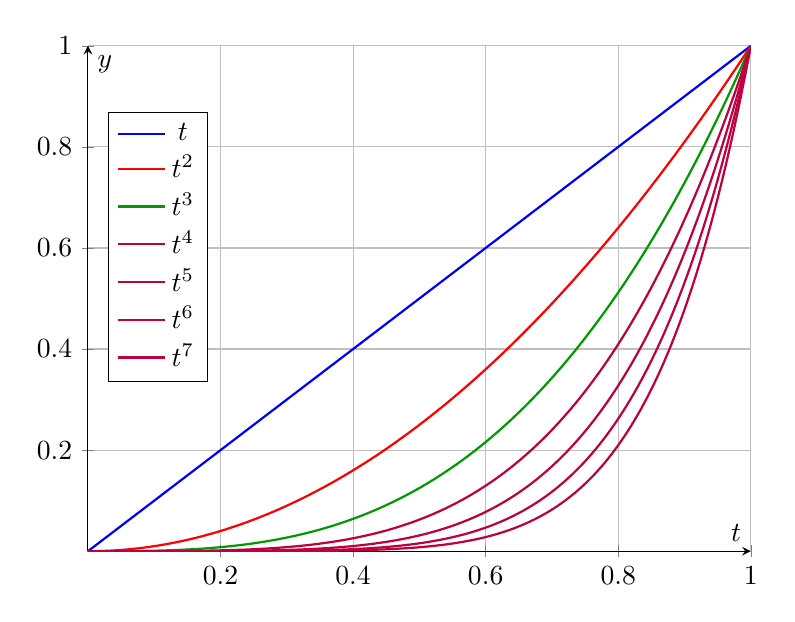
\begin{tikzpicture}
    \begin{axis}[
        axis lines = middle,
        xlabel = {$t$},
        ylabel = {$y$},
        xmin=0, xmax=1,
        ymin=0, ymax=1,
        domain=0:1,
        samples=200,
        legend style={at={(0.03,0.87)},anchor=north west},
        width=10cm,
        height=8cm,
        grid=both
    ]

    \addplot[blue, thick] {x};
    \addlegendentry{$t$}

    \addplot[red, thick] {x^2};
    \addlegendentry{$t^2$}

    \addplot[green!60!black, thick] {x^3};
    \addlegendentry{$t^3$}

    \addplot[purple, thick] {x^4};
    \addlegendentry{$t^4$}

    \addplot[purple, thick] {x^5};
    \addlegendentry{$t^5$}

    \addplot[purple, thick] {x^6};
    \addlegendentry{$t^6$}

    \addplot[purple, thick] {x^7};
    \addlegendentry{$t^7$}

    \end{axis}
    \end{tikzpicture}
    \caption{Gráficas de las funciones $f_n$ para $n\leq 7$.}
    \end{figure}

    \noindent
    Tenemos que para $f:[0,1]\to \mathbb{R}$ dada por:
    \begin{equation*}
        f(t) = \left\{\begin{array}{ll}
            0 & \text{si\ } t\in \left[0,1\right[ \\
            1 & \text{si\ } t = 1
        \end{array}\right. 
    \end{equation*}
    $f_n\to f$ puntualmente, con $f_n$ continua para cada $n\in \mathbb{N}$ y $f$ no es continua.
\end{ejemplo}

\noindent
Diremos que una sucesión de funciones $f_n:I\to \mathbb{R}^d$ es uniformemente de Cauchy si:
\begin{equation*}
    \forall \varepsilon>0~~\exists N\in \mathbb{N} : n,m\geq N \quad \Longrightarrow \quad \|f_n(t) - f_m(t)\| < \varepsilon
\end{equation*}

\noindent
Recordemos además que si una sucesión de funciones $\{f_n\}$ es \textbf{uniformemente de Cauchy} entonces $\{f_n\}$ converge uniformemente a una función $f$.\\

\noindent
Para realizar de forma cómoda el trabajo posterior, conviene tener claro el concepto de sucesión \textbf{parcial} de una sucesión de funciones. Dada una aplicación $\sigma:\mathbb{N}\to \mathbb{N}$ estrictamente creciente, se dice que la sucesión $\{f_{\sigma(n)}\}$ es una sucesión parcial de la sucesión $\{f_n\}$.\\

\noindent
Nos interesa ahora responder a la pregunta de dada una sucesión de funciones, ¿cuándo podemos extraer una parcial que converja uniformemente? La respuesta en $\mathbb{R}$ es clara, basta con que la sucesión esté acotada para poder extraer una sucesión parcial convergente.

\begin{definicion}
    Diremos que una sucesión de funciones $f_n:I\to \mathbb{R}^d$ está \textbf{uniformemente acotada} si:
    \begin{equation*}
        \exists M>0 \quad :\quad  \|f_n(t)\|\leq M \qquad \forall t\in I\quad \forall n\in \mathbb{N}
    \end{equation*}
\end{definicion}

\begin{ejemplo}
    A partir del ejemplo anterior, vemos que tomando $M=1$ tenemos que $\{f_n\}$ es uniformemente acotada, pero no puede tener una parcial que converja uniformemente, pues si existiera una parcial $\{f_{\sigma(n)}\}$ convergente uniformemente tendríamos entonces que $\{f_{\sigma(n)}\}\to f^\ast$ uniformemente para cierta función $f^\ast$ continua en $[0,1]$. En dicho caso, tendríamos que $f_n\to f^\ast$ puntualmente, pero también $f_n\to f$ puntualmente, por lo que $f = f^\ast$, pero tenemos que $f$ no es continua y las funciones $f_{\sigma(n)}$ sí lo son.

    Un ejemplo análogo se podría haber hecho para la sucesión de funciones $\{f_n\}$ cuyas gráficas son la del triángulo cuyo área tiende a $0$, que vimos hace dos ejemplos.
\end{ejemplo}

\begin{definicion}
    Diremos que una sucesión de funciones $f_n:I\to \mathbb{R}^d$ es \textbf{equicontinua\footnote{En realidad el nombre debería ser equi-uniformemente-continua.}} si
    \begin{equation*}
        \forall \varepsilon>0~~\exists \delta>0\quad :\quad \|f_n(t)-f_n(s)\| < \varepsilon \quad \text{si} \quad |t-s|<\delta\quad \forall t,s\in I \qquad \forall n\in \mathbb{N}
    \end{equation*}
\end{definicion}

\begin{ejemplo}
    Consideramos $f_n,g_n:\mathbb{R}\to \mathbb{R}$ dadas por:
    \begin{equation*}
        f_n(t) = \left\{\begin{array}{ll}
            0 & \text{si\ } t<n \\
            t-n & \text{si\ } t\in [n,n+1] \\
            1 & \text{si\ } t>n+1
        \end{array}\right.  \qquad g_n(t) = \left\{\begin{array}{ll}
            0 & \text{si\ } t<0 \\
              nt & \text{si\ } t\in [0,\nicefrac{1}{n}] \\
            1 & \text{si\ } t > \nicefrac{1}{n}
        \end{array}\right. 
    \end{equation*}

    \begin{figure}[H]
        \centering
    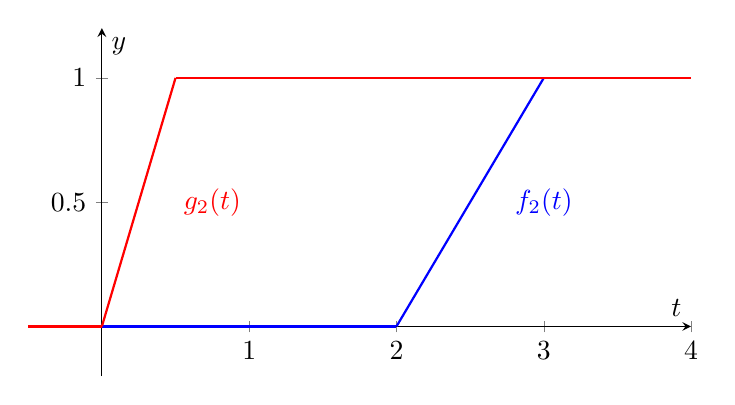
\begin{tikzpicture}
    \begin{axis}[
        axis lines=middle,
        xlabel={$t$},
        ylabel={$y$},
        xmin=-0.5, xmax=4,
        ymin=-0.2, ymax=1.2,
        samples=100,
        width=10cm,
        height=6cm
    ]

    % f_2(t)
    \addplot[blue, thick, domain=-0.5:2] {0};
    \addplot[blue, thick, domain=2:3] {x-2};
    \addplot[blue, thick, domain=3:4] {1};

    % g_2(t)
    \addplot[red, thick, domain=-0.5:0] {0};
    \addplot[red, thick, domain=0:0.5] {2*x};
    \addplot[red, thick, domain=0.5:4] {1};

    \fill[red] (0.75,0.5) node[] {$g_2(t)$};
    \fill[blue] (3,0.5) node[] {$f_2(t)$};

    \end{axis}
    \end{tikzpicture}
    \end{figure}

    \noindent
    Vemos que $\{f_n\}$ es equicontinua. Para ello, basta ver que $f_n$ es lipschitziana para $M=1$, es decir, que:
    \begin{equation*}
        |f_n(t)-f_n(s)| \leq |t-s| \qquad \forall t,s\in \mathbb{R}, \quad \forall n\in \mathbb{N}
    \end{equation*}
    Para ello, bien distinguimos (muchos) casos o notamos que si definimos:
    \begin{equation*}
        h_n(t) = \left\{\begin{array}{ll}
                1 & \text{si\ } t\in [n,n+1] \\
            0 & \text{si\ } t<n \text{\ ó\ } t > n+1
        \end{array}\right. 
    \end{equation*}
    tenemos que:
    \begin{equation*}
        f_n(t) = \int_{0}^{t} h_n(s)~ds  \qquad \forall t\in \mathbb{R}
    \end{equation*}
    Y así obtenemos fácilmente que:
    \begin{equation*}
        \|f_n(s) - f_n(t) \| = \left\|\int_{s}^{t} h(\tau)~d\tau \right\| \leq |t-s|
    \end{equation*}

    \noindent
    Veamos ahora que $\{g_n\}$ no es equicontinua. Para ello, si fuese equicontinua, para $\varepsilon=\nicefrac{1}{3}$ existiría $\delta>0$ tal que
    \begin{equation*}
        |g_n(t) - g_n(s)| < \frac{1}{3}\qquad \forall t,s\in \mathbb{R}, \quad |t-s| < \delta
    \end{equation*}
    Sin embargo, tenemos que:
    \begin{equation*}
        \left|g_n\left(\frac{1}{n}\right)-g_n(0)\right| = 1
    \end{equation*}
    Y existirá $N\in \mathbb{N}$ de forma que para $n\geq N$ se tenga $\frac{1}{n}<\delta$, con lo que tendremos:
    \begin{equation*}
        1 = \left|g_n\left(\frac{1}{n}\right)-g_n(0)\right| < \frac{1}{3}
    \end{equation*}
    Hemos llegado a una contradicción.
\end{ejemplo}

\begin{teo}[Ascoli-Arzelà]
    Sea $I$ un intervalo acotado y sea $f_n:I\to \mathbb{R}^d$ una sucesión de funciones uniformemente acotada y equicontinua, entonces existe una sucesión parcial $\{f_{\sigma(n)}\}$ que converge uniformemente.
\end{teo}

\begin{ejemplo}
    Notemos que en el enunciado del Teorema exigimos que $I$ sea un intervalo acotado, pues si no lo fuera el Teorema es mentira. Para verlo, si tomamos la sucesión de funciones $\{f_n\}$ del ejemplo anterior tenemos que es una sucesión uniformemente acotada y equicontinua pero que no admite una parcial que converja uniformemente.
\end{ejemplo}
